\subsection*{Цель работы}
Измерение длины световой волны интерференционным методом бипризмы Френеля.

\subsection*{Приборы и принадлежности}
В состав экспериментальной установки входят источник света (лампа накаливания) и зелёный светофильтр, установленные в кожухе с вертикальной раздвижной щелью; оптическая скамья с миллиметровой шкалой; бипризма Френеля и окуляр со своей шкалой закрепленные в держателях, которые могут перемещаться вдоль оптической скамьи.

Светофильтр пропускает определенную часть спектра излучения лампы, длину волны которой надо определить в лабораторной работе. Ширину щели можно изменять с помощью винта, находящегося в верхней части оправы пластин щели. Для получения отчетливых интерференционных полос необходимо, чтобы плоскости щели и основания бипризмы были параллельны. Это достигается соответствующим поворотом бипризмы и/или щели. Окуляр служит для наблюдения интерференционной картины. Для измерения расстояния между полосами он снабжен шкалой, цена наименьшего деления которой составляет 1 мм.

\subsection*{Исследуемые закономерности. Методика эксперимента}

В данной работе в качестве интерференционного метода измерений используется метод бипризмы Френеля. Бипризма Френеля состоит из двух одинаковых призм с очень малым преломляющим углом $\theta$, сложенных вместе основаниями и изготовленных как единое целое. Схема получения интерференционной картины с помощью бипризмы Френеля показана на рис. 2.3.

\begin{figure}
    \centering
    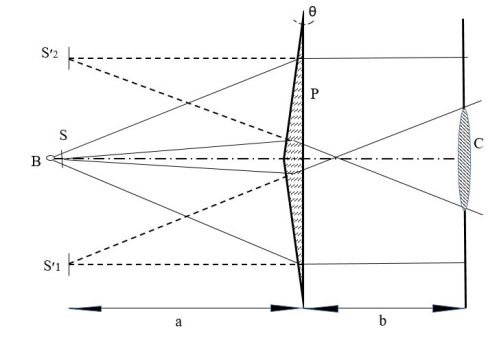
\includegraphics[width=0.5\linewidth]{figs/2.3.png}
    \caption*{Рис. 2.3.}
    \label{fig:2.3.}
\end{figure}

Пучок лучей от источника света B через щель S падает на обе половины бипризмы P, преломляется в них, и за призмой свет распространяется в виде двух когерентных пучков волн с вершинами в мнимых изображениях ${S'}_{1}$ и ${S'}_{2}$ щели S. В области C экрана пучки перекрываются и создают систему параллельных светлых и темных интерференционных полос.

Светлые полосы находятся в тех местах экрана, где лучи, приходящие от источников ${S'}_{1}$ и ${S'}_{2}$, имеют разность хода, равную целому числу длин волн или четному числу полуволн, а темные в тех местах, куда приходят лучи с разностью хода, равной нечетному числу полуволн.

Ширина интерференционной полосы
\begin{equation}
    \Delta x = \frac{(a+b)\lambda_{0}}{d},
\end{equation}
где $a$ и $b$ соответственно расстояния от щели до бипризмы и от бипризмы до экрана; $d$ -- расстояние между мнимыми изображениями источника света.

Для определения расстояния $d$ рассмотрим ход луча, проходящего в верхней половине бипризмы при угле наименьшего отклонения параллельно основанию призмы, т.е. луча SOM (рис. 2.4). В связи с малостью преломляющего угла $\theta$, угол отклонения луча $\delta = {S'}_{2}OS$ тоже мал. Следовательно,

\begin{equation}
    d/2 = {S'}_{2}S = a \cdot \tan \delta \approx a \cdot \delta.
\end{equation}

\begin{figure}[H]
    \centering
    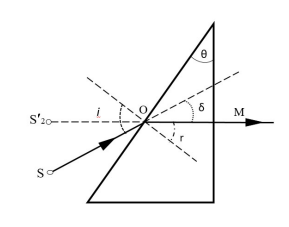
\includegraphics[width=0.5\linewidth]{figs/image.png}
\end{figure}

Для точки O (рис. 2.4) в соответствии с законом преломления света $\sin i / \sin r = n$, где $n$ — показатель преломления материала призмы (стекла); $i$ и $r$ -- углы падения и преломления, соответственно. Вследствие малости углов справедливо соотношение $i = n \cdot r$. Из рис. 2.4 видно, что $r = \theta$ и $i = \delta + r = \delta + \theta$. Тогда $n = i/r = (\delta + \theta) / \theta$, откуда угол отклонения луча $\delta = \theta(n-1)$.

Подставляя $\delta$ в формулу (2.2), получим
\begin{equation}
    d = 2a \cdot \delta = 2a \cdot \theta(n-1).
\end{equation}

Формула (2.3) остается справедливой и при других углах отклонения $\delta$. Из формул (2.1) и (2.2) получим:
$$ \Delta x = (a+b)\lambda_{0} / 2a\theta(n-1), $$
откуда
\begin{equation}
    \lambda_{0} = \frac{2a\theta(n-1)\Delta x}{a+b}.
    \label{eq:2.4}
\end{equation}

Выражение (2.4) показывает, что для нахождения длины световой волны нужно знать расстояние от источника света до экрана $(a+b)$, расстояние от источника света до бипризмы $a$, показатель преломления стекла бипризмы $n$, преломляющий угол бипризмы $\theta$ и ширину интерференционной полосы $\Delta x$. Ширина интерференционной полосы соответствует расстоянию между двумя соседними интерференционными максимумами или минимумами в интерференционной картине распределения интенсивности света. В данной лабораторной работе это расстояние эквивалентно расстоянию $\Delta x$ между наблюдаемыми соседними интерференционными полосами (рис. 2.5).

\begin{figure}[H]
    \centering
    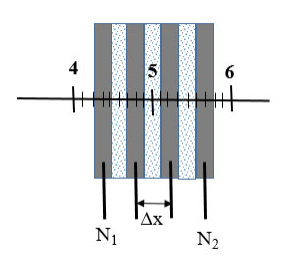
\includegraphics[width=0.5\linewidth]{figs/3.png}
\end{figure}

Оценка этого расстояния производится по формуле
\begin{equation}
    \Delta x = \frac{(N_{2}-N_{1}) \cdot 10c}{m-1},
    \label{eq:2.5}
\end{equation}
где $N_{2}$ и $N_{1}$ -- отсчеты интерференционных полос на окулярной шкале, $c = 0.1$ мм -- цена наименьшего деления окулярной шкалы, с поправочным коэффициентом 10, учитывающим разбиение отсчетов в целых числах на 10 частей, $m$ -- число интерференционных полос между отсчетами $N_{2}$ и $N_{1}$. В примере на рис. 2.5 $m = 4$.


\newpage
\subsection*{Указания по выполнению эксперимента}
\begin{enumerate}
    \item Включить лампу и убедиться, что свет от нее падает симметрично на обе половины бипризмы. Для этого нужно расширить щель и приложить к бипризме кусок белой бумаги. Если свет падает на бипризму несимметрично относительно ее ребра, то следует переместить бипризму вправо или влево.
    \item Поместить окуляр на максимальное расстояние от щели. Сузить щель, поставить ее параллельно ребру бипризмы и поместить бипризму на расстоянии $a$ от щели (примерно посредине между щелью и окуляром). Положения щели, бипризмы и окуляра отмечены рисками на основаниях их держателей. Расстояния $a$ и $(a+b)$ определяются по измерительной шкале на оптической скамье и задаются преподавателем.
    \item Проверить, достаточно ли четко видны деления шкалы окуляра. Слегка перемещая трубку окуляра вперёд и назад, добиться четкого изображения шкалы.
    \item Рассмотреть интерференционные полосы через окуляр и небольшим вращением бипризмы вокруг вертикальной и горизонтальной осей, а также регулируя ширину щели, добиться наибольшей четкой интерференционной картины.
    \item Ориентируясь на первую и последнюю наблюдаемые светлые или темные полосы интерференционной картины, определить по шкале окуляра положения $N_{1}$ и $N_{2}$ этих полос. Записать значения $m$, $a$, $(a+b)$, $N_{1}$ и $N_{2}$ в таблицу протокола наблюдений.
    \item Выполнить эксперименты, аналогичные п. 5, еще 4 раза при одном и том же расстоянии $(a+b)$, изменяя расстояние $a$ от щели до бипризмы (приближая или удаляя держатель бипризмы с шагом, задаваемым преподавателем, относительно среднего положения бипризмы). Записать результаты наблюдений по аналогии с п. 5 в таблицу для каждого значения $a$.
    \item Записать в протокол наблюдений значение $c = 0.1$ мм цены наименьшего деления шкалы окуляра, а также значения показателя преломления стекла $n$ и преломляющего угла $\theta$ бипризмы, указанные на панели экспериментальной установки.
\end{enumerate}




\newpage
\thispagestyle{empty}
\centeredsection{ПРОТОКОЛ НАБЛЮДЕНИЙ}



\noindent
\textbf{Таблица 1. Константы эксперимента}

\noindent
\begin{tabularx}{\textwidth}{| C | C | C | C |}
    \hline
        $c,~\frac{\text{мм}}{\text{дел}}$ & $\theta,~\text{Рад}$ & $n$ & $N_{max}$ \\
    \hline
        0.1 & 0.011 & 1.52 & 15 \\
    \hline
\end{tabularx}



\vspace{1cm}
\noindent
\textbf{Таблица 2. Измерения}

\noindent
\begin{tabularx}{\textwidth}{| C | C | C | C | C |}
    \hline
        № & $a,~\text{мм}$ & $N_1$,~\text{дел} & $N_2$,~\text{дел} & $m$ \\
    \hline
        1 & 300 & 38 & 48 & 14 \\
    \hline
        2 & 310 & 37 & 48 & 13 \\
    \hline
        3 & 290 & 37 & 49 & 14 \\
    \hline
        4 & 295 & 38 & 48 & 13 \\
    \hline
        5 & 305 & 38 & 49 & 13 \\
    \hline
\end{tabularx}

\vfill
\noindent
Рахметов А. Р., гр. 4494 ~~\hrulefill~~ «\rule{1cm}{0.4pt}» \rule{3cm}{0.4pt} 20\rule{0.75cm}{0.4pt} г.





\newpage
\centeredsection{ОБРАБОТКА РЕЗУЛЬТАТОВ}

\section*{Задание 1.}
\begin{quote}
    \textit{
        Используя результаты наблюдений, значения $с$, $m$, $N_2$ и $N_1$ для каждого опыта, исходя из формулы (\ref{eq:2.5}), рассчитать расстояние $\Delta x$ между двумя интерференционными полосами (светлыми или темными) для каждого из пяти наблюдений.
    }
\end{quote}

$\Delta x = \frac{(N_{2}-N_{1}) \cdot 10c}{m-1}$.
Для №1:
$
    \Delta x = \frac{
        (48-38) \cdot 10 \cdot 0,1\text{мм}
    }{
        14-1
    }
    \approx
    0,7692\text{мм}
$
и так далее:

\begin{table}[H]
    \centering
    \begin{tabular}{ c c }
        № & $\Delta x,~\text{мм}$ \\
        \midrule
        1 & 0,7692 \\
        2 & 0,9167 \\
        3 & 0,9231 \\
        4 & 0,8333 \\
        5 & 0,9167 \\
    \end{tabular}
\end{table}


\section*{Задание 2.}
\begin{quote}
    \textit{
        По формуле (\ref{eq:2.4}) для каждого из пяти наблюдений вычислить длину волны $\lambda$ источника света после прохождения светофильтра.
    }
\end{quote}

$\lambda_{0} = \frac{2a\theta(n-1)\Delta x}{a+b}$.
Для №1, где $a + b = 550\text{мм}$:
$
    \lambda_{0} = \frac{
        2\cdot 300\text{мм} \cdot 0.011 \cdot (1,52-1)\cdot 0,7692\text{мм}
    }{
        550\text{мм}
    }
    \approx
    0,000480\text{мм} = 480\text{нм}
$ и так далее:

\begin{table}[H]
    \centering
    \begin{tabular}{ c c }
        № & $\lambda,~\text{нм}$ \\
        \midrule
        1 & 480 \\
        2 & 591 \\
        3 & 557 \\
        4 & 511 \\
        5 & 582 \\
    \end{tabular}
\end{table}

\section*{Задание 3.}
\begin{quote}
    \textit{
        Рассчитать среднее значение длины волны $\overline\lambda$ и погрешность измерений $\Delta\overline\lambda$. Представить результат измерения в округленном виде. Сделать выводы по работе.
    }
\end{quote}

Найдем $\overline{\lambda}\pm\Delta\overline{\lambda}$:
\begin{enumerate}
    \item $$\overline{\lambda} = \frac15\sum_{i=1}^5\lambda_i=544,1$$
    \item $\delta\lambda_i = \lambda_i - \overline\lambda$
    
        \begin{table}[H]
            \centering
            \begin{tabular}{| c | c | c | c | c | c |}
                \hline
                $\delta\lambda_i$ & -64,1 & 46,9 & 12,7 & -32,8 & 37,4\\
                \hline
            \end{tabular}
        \end{table}
        $$\sum\limits_{i=1}^5\delta\lambda_i = 0$$
        $$S_{\overline{\lambda}} = \sqrt{ \frac{ \sum\limits_{i=1}^5(\delta\lambda_i)^2 }{5\cdot4} } = 21,16$$
    \item 
        $$t_{95\%,5}=2,78$$
        $$\Delta\lambda=t_{P,N}\cdot S_{\overline\lambda} = 2,78 \cdot 21,16 = 58,82$$
    \item 
        $$\lambda = \overline\lambda \pm \Delta\overline\lambda.$$
        $$\lambda = (544,1 \pm 58,82)~\text{нм}$$
        $$\framebox{
            \lambda = (540 \pm 60)~\text{нм}
        }$$
\end{enumerate}



\section*{Выводы}
В результате пяти серий измерений и последующей статистической обработки данных была найдена $\lambda = (540 \pm 60)$ нм. Измерения проводились при доверительной вероятности $P=0,95$.

Относительная погрешность
$$\varepsilon = \frac{\Delta\overline{\lambda}}{\overline{\lambda}} \times 100\% = \frac{60}{540} \times 100\% \approx 11,1\% $$
является приемлемой.

Измеренное значение длины волны $\lambda = 540 \text{ нм}$ лежит в диапазоне длин волн зелёного света ($495-570$ нм), что подтверждает корректность использования зелёного светофильтра в установке.

В результате удалось достичь цель работы: длина волны света, прошедшего через светофильтр, определена интерференционным методом бипризмы Френеля.

\newpage
\centeredsection{Вопросы}
\section*{Вопрос 1 (№19).}
\begin{quote}
    \textit{Сформулируйте принцип суперпозиции волн.}
\end{quote}

Принцип суперпозиции утверждает, что если в среде одновременно распространяется несколько волн, то результирующее смещение среды в любой точке и в любой момент времени равно векторной сумме смещений, которые создавала бы каждая из волн в отдельности.

\begin{equation*}
    \vec{E} = \sum_{i=1}^{n} \vec{E}_i
\end{equation*}



\section*{Вопрос 2 (№37).}
\begin{quote}
    \textit{Какова интерференция при отражении света от плоскопараллельной пластинки? Покажите ход лучей. Рассчитайте оптическую разность хода.}
\end{quote}
\begin{figure}[H]
    \centering
    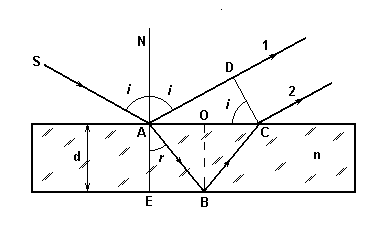
\includegraphics[width=0.5\linewidth]{figs/interferenc.png}
\end{figure}
Лучи (1) и (2) являются когерентными (т.е. колебания происходят синхронно; т.к. они произошли от одного исходного луча) и распространяются параллельно друг другу. Их интерференция наблюдается в плоскости, перпендикулярной лучам (1) и (2).

Оптическая разность хода (разность хода; $\Delta$) --- это разница между оптическими длинами путей, пройденных двумя когерентными световыми волнами от общего источника до одной и той же точки: $\Delta = l_2-l_1=l_1-l_2$; $\Delta = m\lambda$ (для max); $\Delta = (m+\frac12)\lambda$ (для min), где $l_\text{опт}=n\cdot l_\text{геом}$.

Оптическая длина пути --- расстояние, на которое свет распространился бы в вакууме за время его прохождения между данными двумя точками.

Для примера выше оптическая разность хода будет равна: $\Delta=2nd\cos(i')+\frac{\lambda}2$.

\newpage
\centeredsection{ИДЗ №33}
\begin{quote}
    Пучок монохроматических ($\lambda= 600$ нм) световых волн падает под углом $\alpha= 30^\circ$ на находящуюся в воздухе мыльную плёнку ($n = 1,30$). При какой наименьшей толщине $d$ плёнки отражённые световые волны будут: 1) максимально ослаблены интерференцией; 2) максимально  усилены?
\end{quote}
\begin{figure}[H]
    \centering
    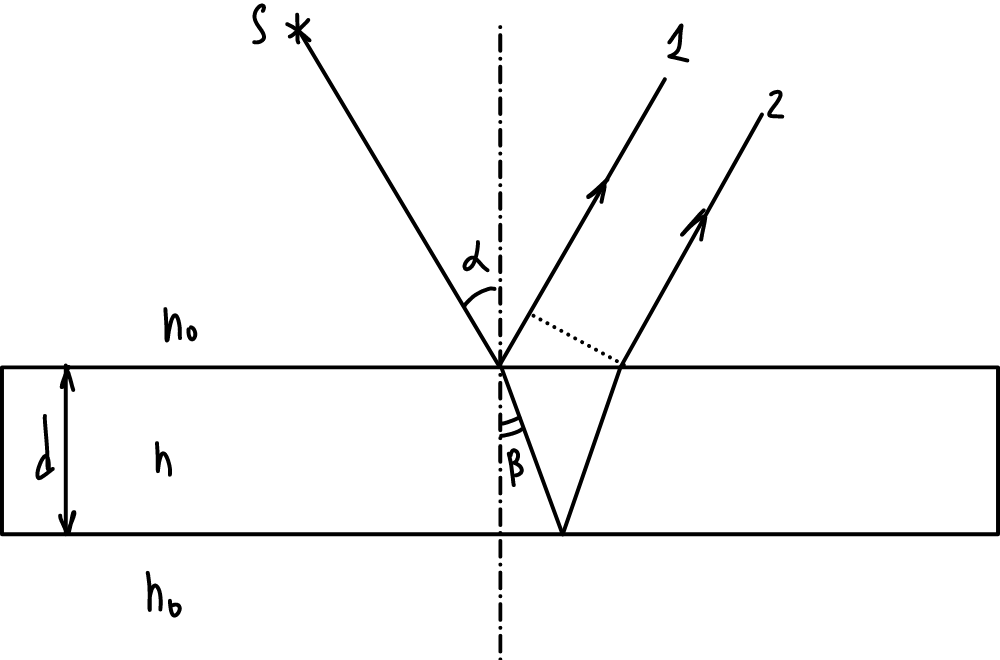
\includegraphics[width=0.5\linewidth]{figs/IMG_20250928_220659_551.jpg}
\end{figure}

\begin{enumerate}
    \item Рассчитаем $\cos\beta$
        $$n_0\sin\alpha=n\sin\beta\Rightarrow\sin\beta=\frac{n_0\sin\alpha}{n}=\frac{1\cdot\sin(30^\circ)}{1,3}=\frac{5}{13}$$

        $$\cos\beta=\sqrt{1-\sin^2\beta}=\sqrt{\frac{144}{169}}=\frac{12}{13}$$

        $$\cos\beta=\frac{12}{13}$$

    \item Найдем разность хода
        $$l_1=\frac\lambda2;\qquad l_2=2nd\cos\beta;\qquad \Delta=l_2-l_1$$
        $$\Delta=2nd\cos\beta-\frac{\lambda}{2}$$
    \item Максимальное ослабление ($\Delta=(m+\frac12)\lambda$)
        $$2nd\cos\beta-\frac{\lambda}{2} = (m+\frac12)\lambda$$
        $$2nd\cos\beta = (m+\frac12)\lambda + \frac{\lambda}{2}$$
        $$2nd\cos\beta = (m+1)\lambda, m\in\mathbb{Z} \Rightarrow m+1\equiv m$$
        $$2nd\cos\beta = m\lambda$$
        $$d = \frac{m\lambda}{2n\cos\beta},~~d_{min}\text{ при } m=1$$
        $$d = \frac{\lambda}{2n\cos\beta}$$
        $$d_{min} = \frac{600\text{ нм}}{2\cdot 1,3 \cdot \frac{12}{13}}=250\text{ нм}$$
        $$\boxed{d_{min, \text{ослабление}} = 250\text{ нм}}$$
    \item Максимальное усиление ($\Delta=m\lambda$)
        $$2nd\cos\beta-\frac{\lambda}{2} = m\lambda$$
        $$2nd\cos\beta = m\lambda + \frac{\lambda}{2}$$
        $$2nd\cos\beta = (m+\frac12)\lambda$$
        $$d = \frac{(m+\frac12)\lambda}{2n\cos\beta},~~d_{min}\text{ при } m=0$$
        $$d_{min} = \frac{\frac12\lambda}{2n\cos\beta}$$
        $$d_{min} = \frac{\frac{1}{2}\cdot600\text{ нм}}{2\cdot 1,3 \cdot \frac{12}{13}}=125\text{ нм}$$
        $$\boxed{d_{min, \text{усиление}} = 125\text{ нм}}$$
        
\end{enumerate}
